\documentclass[14pt]{extbook}
\usepackage{multicol, enumerate, enumitem, hyperref, color, soul, setspace, parskip, fancyhdr} %General Packages
\usepackage{amssymb, amsthm, amsmath, latexsym, units, mathtools} %Math Packages
\everymath{\displaystyle} %All math in Display Style
% Packages with additional options
\usepackage[headsep=0.5cm,headheight=12pt, left=1 in,right= 1 in,top= 1 in,bottom= 1 in]{geometry}
\usepackage[usenames,dvipsnames]{xcolor}
\usepackage{dashrule}  % Package to use the command below to create lines between items
\newcommand{\litem}[1]{\item#1\hspace*{-1cm}\rule{\textwidth}{0.4pt}}
\pagestyle{fancy}
\lhead{Progress Quiz 1}
\chead{}
\rhead{Version A}
\lfoot{4082-7053}
\cfoot{}
\rfoot{test}
\begin{document}

\begin{enumerate}
\litem{
Write the equation of the line in the graph below in Standard form $Ax+By=C$. Then, choose the intervals that contain $A, B, \text{ and } C$.
\begin{center}
    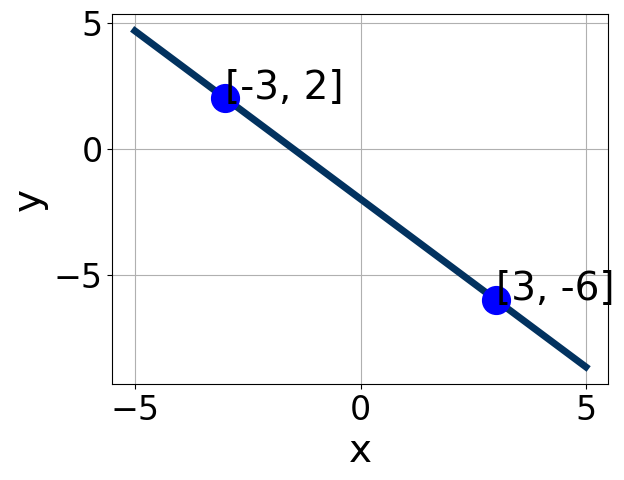
\includegraphics[width=0.5\textwidth]{../Figures/linearGraphToStandardA.png}
\end{center}
\begin{enumerate}[label=\Alph*.]
\item \( A \in [0.6, 4.9], \hspace{3mm} B \in [1.76, 2.67], \text{ and } \hspace{3mm} C \in [-3, 4] \)
\item \( A \in [-4.9, -1.8], \hspace{3mm} B \in [1.76, 2.67], \text{ and } \hspace{3mm} C \in [-3, 4] \)
\item \( A \in [0.6, 4.9], \hspace{3mm} B \in [-2.59, -1.75], \text{ and } \hspace{3mm} C \in [-3, 4] \)
\item \( A \in [-2.9, 0.5], \hspace{3mm} B \in [-0.39, 1.35], \text{ and } \hspace{3mm} C \in [-3, 4] \)
\item \( A \in [-2.9, 0.5], \hspace{3mm} B \in [-1.73, -0.72], \text{ and } \hspace{3mm} C \in [-3, 4] \)

\end{enumerate} }
\litem{
Find the equation of the line described below. Write the linear equation as $ y=mx+b $ and choose the intervals that contain $m$ and $b$.\[ \text{Perpendicular to } 6 x + 7 y = 7 \text{ and passing through the point } (-5, -9). \]\begin{enumerate}[label=\Alph*.]
\item \( m \in [1.1, 1.9] \hspace*{3mm} b \in [-4.49, -3.25] \)
\item \( m \in [1.1, 1.9] \hspace*{3mm} b \in [2.38, 3.72] \)
\item \( m \in [-1, 1.1] \hspace*{3mm} b \in [-3.51, -2.36] \)
\item \( m \in [1.1, 1.9] \hspace*{3mm} b \in [-3.51, -2.36] \)
\item \( m \in [-1.9, -1] \hspace*{3mm} b \in [-14.96, -14.51] \)

\end{enumerate} }
\litem{
Solve the equation below. Then, choose the interval that contains the solution.\[ -3(5x -7) = -2(-11x -19) \]\begin{enumerate}[label=\Alph*.]
\item \( x \in [-2.59, -0.59] \)
\item \( x \in [-0.41, 2.59] \)
\item \( x \in [-8.43, -6.43] \)
\item \( x \in [-1.46, 1.54] \)
\item \( \text{There are no real solutions.} \)

\end{enumerate} }
\litem{
Find the equation of the line described below. Write the linear equation as $ y=mx+b $ and choose the intervals that contain $m$ and $b$.\[ \text{Parallel to } 8 x - 7 y = 15 \text{ and passing through the point } (-4, -8). \]\begin{enumerate}[label=\Alph*.]
\item \( m \in [1.01, 1.46] \hspace*{3mm} b \in [-3.58, -3.34] \)
\item \( m \in [1.01, 1.46] \hspace*{3mm} b \in [2.98, 3.57] \)
\item \( m \in [-1.19, -1.09] \hspace*{3mm} b \in [-12.74, -12.01] \)
\item \( m \in [1.01, 1.46] \hspace*{3mm} b \in [-4.69, -3.53] \)
\item \( m \in [0.77, 0.99] \hspace*{3mm} b \in [-3.58, -3.34] \)

\end{enumerate} }
\litem{
Write the equation of the line in the graph below in Standard form $Ax+By=C$. Then, choose the intervals that contain $A, B, \text{ and } C$.
\begin{center}
    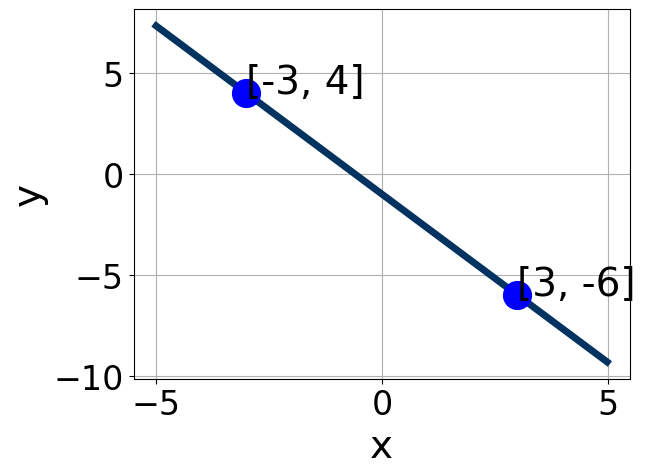
\includegraphics[width=0.5\textwidth]{../Figures/linearGraphToStandardCopyA.png}
\end{center}
\begin{enumerate}[label=\Alph*.]
\item \( A \in [3, 8], \hspace{3mm} B \in [-6, -3.9], \text{ and } \hspace{3mm} C \in [-3, 6] \)
\item \( A \in [-8, -3], \hspace{3mm} B \in [3.2, 6.6], \text{ and } \hspace{3mm} C \in [-3, 6] \)
\item \( A \in [-2.25, 0.75], \hspace{3mm} B \in [-2.8, -0.5], \text{ and } \hspace{3mm} C \in [-3, 6] \)
\item \( A \in [3, 8], \hspace{3mm} B \in [3.2, 6.6], \text{ and } \hspace{3mm} C \in [-3, 6] \)
\item \( A \in [-2.25, 0.75], \hspace{3mm} B \in [0.4, 3.3], \text{ and } \hspace{3mm} C \in [-3, 6] \)

\end{enumerate} }
\litem{
Solve the linear equation below. Then, choose the interval that contains the solution.\[ \frac{5x + 8}{6} - \frac{6x + 4}{7} = \frac{-3x -3}{4} \]\begin{enumerate}[label=\Alph*.]
\item \( x \in [-5.1, -3.3] \)
\item \( x \in [-11.3, -9.6] \)
\item \( x \in [-3.2, -1.2] \)
\item \( x \in [-1.3, 0.2] \)
\item \( \text{There are no real solutions.} \)

\end{enumerate} }
\litem{
Solve the equation below. Then, choose the interval that contains the solution.\[ -11(-10x -9) = -18(-14x -7) \]\begin{enumerate}[label=\Alph*.]
\item \( x \in [-1.05, -0.31] \)
\item \( x \in [-0.28, 0.45] \)
\item \( x \in [0.76, 2.33] \)
\item \( x \in [-2.51, -1.31] \)
\item \( \text{There are no real solutions.} \)

\end{enumerate} }
\litem{
First, find the equation of the line containing the two points below. Then, write the equation as $ y=mx+b $ and choose the intervals that contain $m$ and $b$.\[ (-11, 9) \text{ and } (-9, -4) \]\begin{enumerate}[label=\Alph*.]
\item \( m \in [-12.5, -3.5] \hspace*{3mm} b \in [3, 6] \)
\item \( m \in [-12.5, -3.5] \hspace*{3mm} b \in [59.5, 68.5] \)
\item \( m \in [-12.5, -3.5] \hspace*{3mm} b \in [-63.5, -59.5] \)
\item \( m \in [2.5, 12.5] \hspace*{3mm} b \in [51.5, 60.5] \)
\item \( m \in [-12.5, -3.5] \hspace*{3mm} b \in [20, 29] \)

\end{enumerate} }
\litem{
Solve the linear equation below. Then, choose the interval that contains the solution.\[ \frac{5x + 5}{8} - \frac{9x -7}{6} = \frac{-3x -3}{7} \]\begin{enumerate}[label=\Alph*.]
\item \( x \in [3.97, 7.97] \)
\item \( x \in [32.6, 36.6] \)
\item \( x \in [1.22, 3.22] \)
\item \( x \in [-2.25, 1.75] \)
\item \( \text{There are no real solutions.} \)

\end{enumerate} }
\litem{
First, find the equation of the line containing the two points below. Then, write the equation as $ y=mx+b $ and choose the intervals that contain $m$ and $b$.\[ (10, 9) \text{ and } (6, -2) \]\begin{enumerate}[label=\Alph*.]
\item \( m \in [-1.25, 3.75] \hspace*{3mm} b \in [-12, -2] \)
\item \( m \in [-1.25, 3.75] \hspace*{3mm} b \in [17.5, 20.5] \)
\item \( m \in [-6.75, -1.75] \hspace*{3mm} b \in [10.5, 16.5] \)
\item \( m \in [-1.25, 3.75] \hspace*{3mm} b \in [-3, 5] \)
\item \( m \in [-1.25, 3.75] \hspace*{3mm} b \in [-19.5, -14.5] \)

\end{enumerate} }
\end{enumerate}

\end{document}